\begin{table}[h!]
    \caption{Resultados da calibração das leituras de \acrshort{mp10} do sensor OPC-N3}
    \centering
    \begin{tabularx}{0.95\textwidth}[h!]{
        >{\raggedright\hsize=.4\hsize\arraybackslash}X
        >{\raggedright\hsize=.6\hsize\arraybackslash}X 
        >{\raggedright\hsize=.6\hsize\arraybackslash}X
        >{\raggedright\hsize=.7\hsize\arraybackslash}X 
        >{\raggedright\hsize=.6\hsize\arraybackslash}X 
        >{\raggedright\hsize=.3\hsize\arraybackslash}X }
        \hline
        Var. & Modelo & R2 & RMSE & MAE & $\rho$\\ [0.5ex]
        \hline
        \acrshort{mp10} & \textbf{MLP}: & -0.05 ± 0.036 & -9.77 ± 0.75 & -7.41 ± 0.49 & 0.18 \\ [0.5ex]
           & \textbf{MLR} & -0.01 ± 0.03 & -9.57 ± 0.98 & -7.26 ± 0.62 & 0.17 \\ [0.5ex]
           & \textbf{KNN:} & -0.14 ± 0.07 & -10.18 ± 0.62 & -7.71 ± 0.45 & 0.13 \\ [0.5ex]
           & \textbf{RF:} & -0.19 ± 0.11 & -10.33 ± 0.52 & -7.80 ± 0.40 & 0.22\\ [0.5ex]
        \hline
        \acrshort{mp10}, T & \textbf{MLP:} & -0.29 ± 0.27 & -10.68 ± 0.96 & -8.33 ± 0.78 & 0.47 \\ [0.5ex]
              & \textbf{MLR:} & 0.10 ± 0.08 & -9.04 ± 1.12 & -6.73 ± 0.69 & 0.37 \\ [0.5ex]
              & \textbf{KNN:} & -0.02 ± 0.09 & -9.57 ± 0.46 & -7.29 ± 0.27 & 0.45 \\ [0.5ex]
              & \textbf{RF:} & -0.17 ± 0.27 & -10.12 ± 0.32 & -7.89 ± 0.28 & 0.46 \\ [0.5ex]
        \hline
    \end{tabularx}
    \label{tab:data-pm10-calib-results}
\end{table}

% ----------------------------------------------------------
\section{Correção das leituras de MP10 do sensor OPC-N3 com as medições de referência}
% ----------------------------------------------------------

A partir dos dados de referência e das leituras de concentração e temperatura adquiridas pelo monitor em questão, foi realizada uma busca em grid para encontrar as melhores combinações de parâmetros e variáveis de entrada a modelos de regressão. As variáveis que foram testadas como entrada foram as leituras de concentração de \acrshort{mp10} do sensor OPC-N3 e a temperatura no interior da câmara de medição. Como modelos de regressão foram testados: o Perceptron Multicamadas (MLP), a Regressão Linear Multivariada (MLR), os K Vizinhos mais Próximos (KNN) e as Florestas Aleatórias (RF). Na Tabela \ref{tab:data-pm10-calib-results} resumem-se os melhores modelos encontrados pela busca em \textit{grid} para calibrar as leituras do sensor OPC-N3. Os mesmos resultados são ilustrados graficamente na Figura \ref{fig:data-pm10-models-performance} que apresenta o desempenho dos modelos e as variáveis de entrada considerando os valores de r2, RMSE e MAE.

\begin{figure}[h!]
    \centering
    \caption{Resultados dos modelos de calibração aplicados as leituras de \acrshort{mp10} do sensor OPC-N3}
    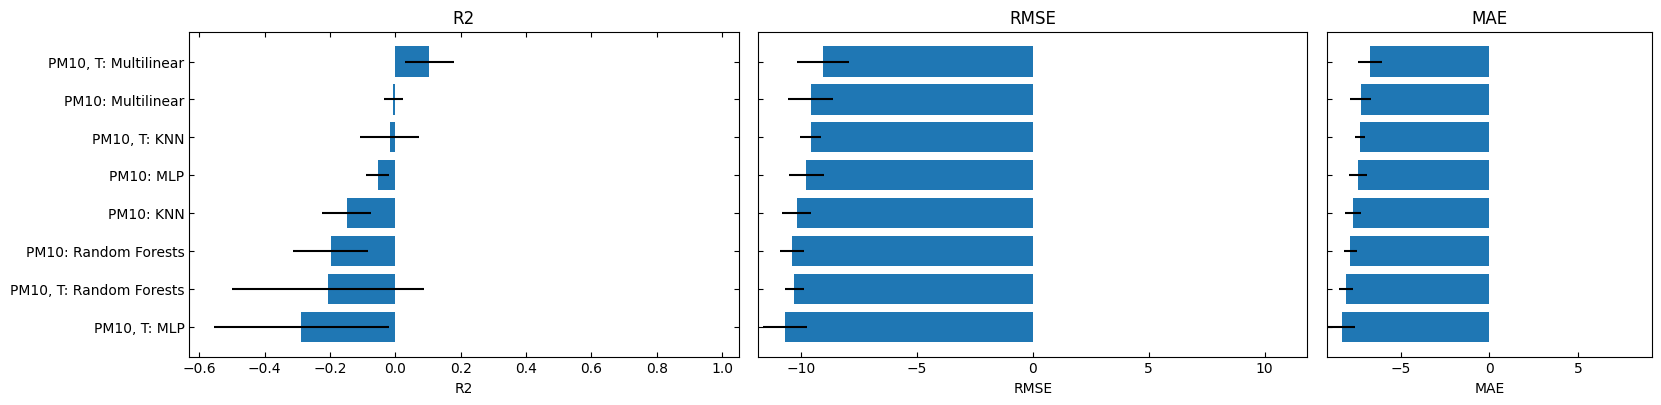
\includegraphics[width=0.95\textwidth]{chapters/4-CALIBRAÇÃO MÚLTIPLOS SENSORES/Figuras/pm10-models-performance.png}
    \label{fig:data-pm10-models-performance}
\end{figure}

\begin{figure}[h!]
    \centering
    \caption{Gráfico de dispersão das leituras do sensor de \acrshort{mp10} do OPC-N3 e a estação de referência após aplicar modelos de regressão considerando a temperatura}
    \begin{subfigure}{0.49\textwidth}
        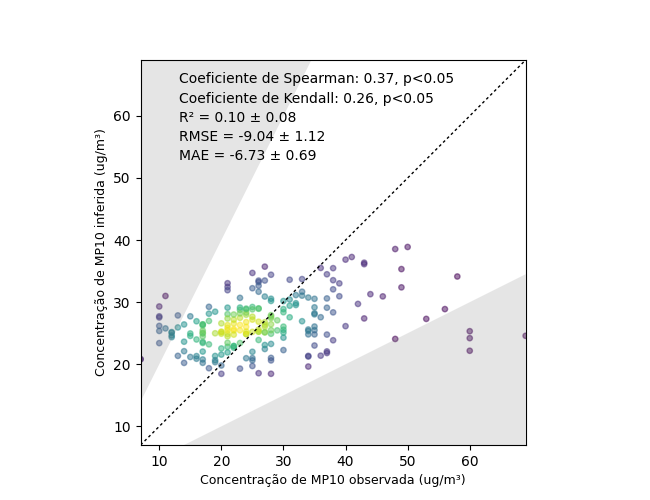
\includegraphics[width=\textwidth]{chapters/4-CALIBRAÇÃO MÚLTIPLOS SENSORES/Figuras/pm10-T-ML-Regression.png}
        \caption{Utilizando uma regressão linear multivariada considerando a temperatura obteve-se um R2 de 0.10 e $\rho$ de 0.37}
        \label{fig:data-pm10-T-reference-corr-MLR}
    \end{subfigure}
    \hfill
    \begin{subfigure}{0.49\textwidth}
        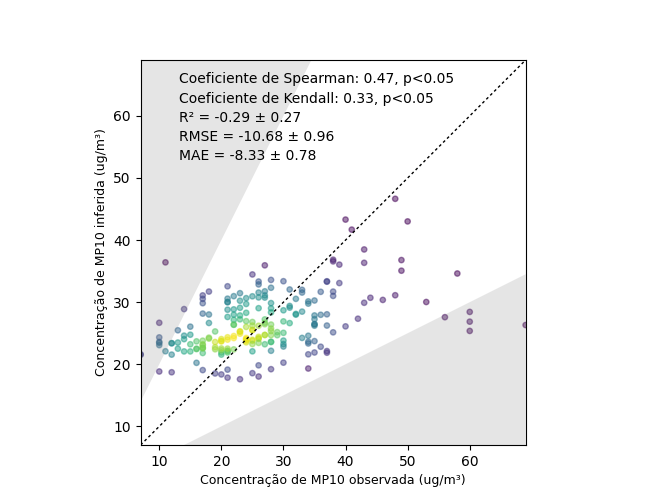
\includegraphics[width=\textwidth]{chapters/4-CALIBRAÇÃO MÚLTIPLOS SENSORES/Figuras/pm10-T-MLP-Regression.png}
        \caption{Utilizando uma rede neural Perceptron Multicamadas considerando a temperatura obtiveram-se valores de $\rho$ de 0.47 e 0.33}
        \label{fig:data-pm10-T-reference-corr-MLP}
    \end{subfigure}
\end{figure}

Como se observa, apenas o modelo de regressão linear com variáveis independentes temperatura e concentração medida pelo sensor OPC-N3 conseguiu explicar a variância na variável dependente, i.e. a concentração real. Os valores de R2 obtidos nas validações cruzadas realizadas para este modelo foram de 0.10 ± 0.08, e os coeficientes de correlação de Spearman e Kendall entre a concentração inferida na calibração e a concentração real foram de 0.37 e 0.26 respectivamente. Os erros RMSE e MAE estiveram próximos de 10 \(\mu g/m^3\), que é um valor relativamente baixo considerando a diferença elevada entre os valores de referência e as leituras do sensor (aproximadamente 10 vezes). De modo geral, os modelos não lineares que incluíram a temperatura como variável dependente, apresentaram melhorias na correlação entre a concentração real e a medida pelo sensor, com coeficientes de correlação de até 0.47. As Figuras \ref{fig:data-pm10-T-reference-corr-MLR} e \ref{fig:data-pm10-T-reference-corr-MLP} apresentam os resultados ao aplicar o modelo de regressão linear considerando leituras do sensor e temperatura e ao aplicar uma rede neural Perceptron Multicamadas considerando as mesmas variáveis de entrada.

\begin{figure}[h!]
    \centering
    \caption{Desempenho dos modelos de regressão aplicados para inferir as leituras de concentração de \acrshort{mp10} medidas pela estação de referência}
    \begin{subfigure}{0.9\textwidth}
        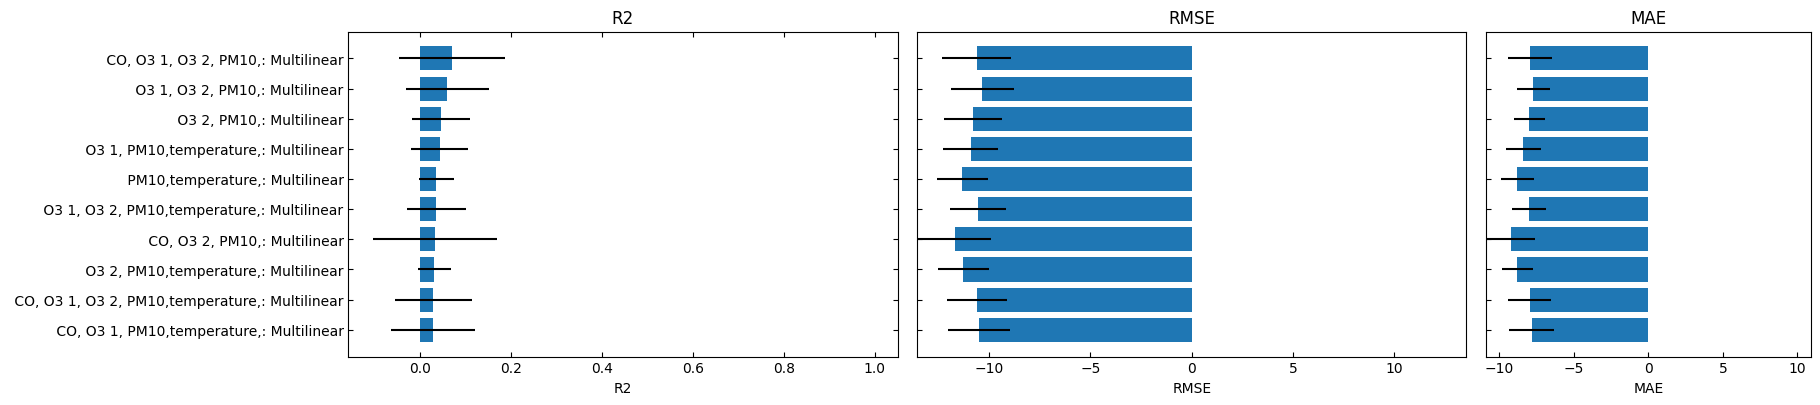
\includegraphics[width=\textwidth]{chapters/4-CALIBRAÇÃO MÚLTIPLOS SENSORES/Figuras/pm10-all-models-performance.png}
        \caption{Valores de R2, RMSE e MAE obtidos pelos 10 modelos com maiores valores de R2}
        \label{fig:data-pm10-all-models-performance}
    \end{subfigure}
    \begin{subfigure}{0.9\textwidth}
        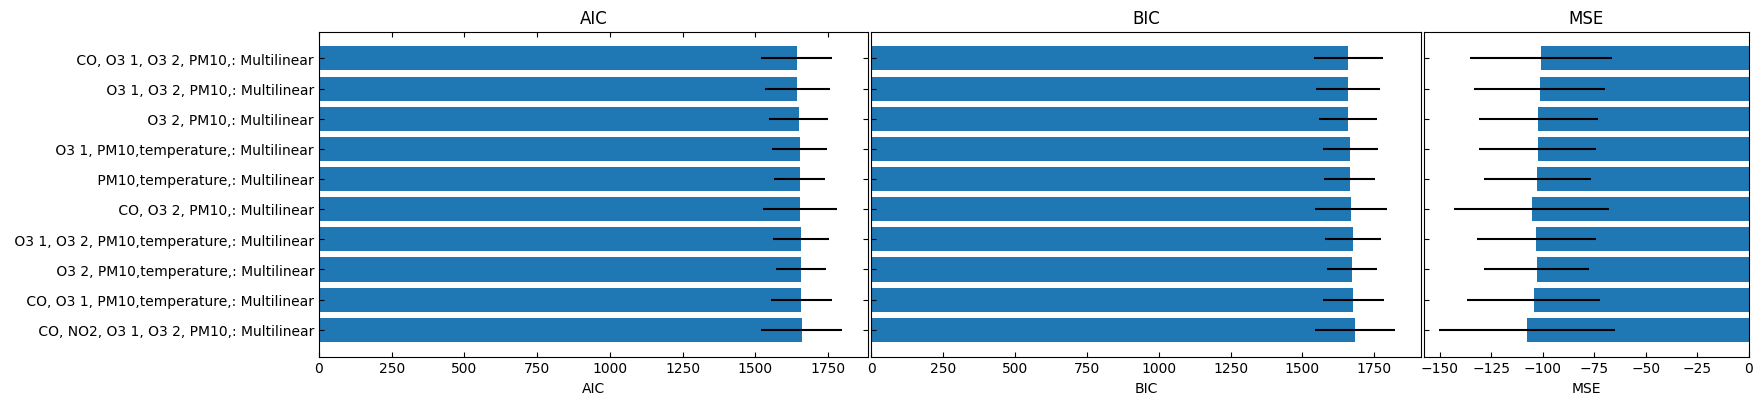
\includegraphics[width=\textwidth]{chapters/4-CALIBRAÇÃO MÚLTIPLOS SENSORES/Figuras/pm10-all-models-complexity.png}
        \caption{Modelos com menores valores de \acrshort{aic} e \acrshort{bic}}
        \label{fig:data-pm10-all-models-comlexity}
    \end{subfigure}
    \label{fig:data-pm10-all-models-performance-comlexity}
\end{figure}

% ----------------------------------------------------------
\section{Cálculo da concentração de MP10 a partir das leituras do arranjo de sensores de gases}
% ----------------------------------------------------------

A Figura \ref{fig:data-pm10-all-models-performance} apresenta os valores de R2 dos 10 melhores modelos de calibração calculados para as leituras de \acrshort{mp10}. Observa-se que os valores de R2 desses 10 modelos apresentaram valores de R2 em média positivos, com valores mínimos e máximos oscilando entre -0.1 e 0.2, todos obtidos a partir de regressões lineares. Com relação as variáveis de entrada observa-se maior variabilidade do que nos casos analisados anteriormente, mas em geral destaca-se a presença de sensores de \acrshort{o3} em 9 dos modelos e em segundo lugar da temperatura, presente em 6. Nenhum dos modelos incluiu leituras do sensor NO2-B43F. Com relação à complexidade dos modelos (Figura \ref{fig:data-pm10-all-models-performance-comlexity}) observa-se bastante coincidência com ranqueamento de R2. As Figuras \ref{fig:data-co-o31-o31-pm10-reference-PM10-corr-MLR} e \ref{fig:data-o31-o32-pm10-reference-PM10-corr-RF} mostram os resultados obtidos com os dois modelos com maior R2 médio, i.e.: regressões lineares com variáveis de entrada leituras de sensores CO-B4, OX-B431 (1 e 2) e sensor de \acrshort{mp10} OPC-N3, e leituras de sensores OX-B431 (1 e 2) e sensor de \acrshort{mp10} OPC-N3, respectivamente. As figuras mostram gráficos de dispersão entre os dados calibrados por esses modelos e as leituras de referência.

\begin{figure}[h]
    \centering
    \caption{Gráfico de dispersão das leituras do múltiplos sensores e a estação de referência para medição de \acrshort{mp10}}
    \begin{subfigure}{0.49\textwidth}
        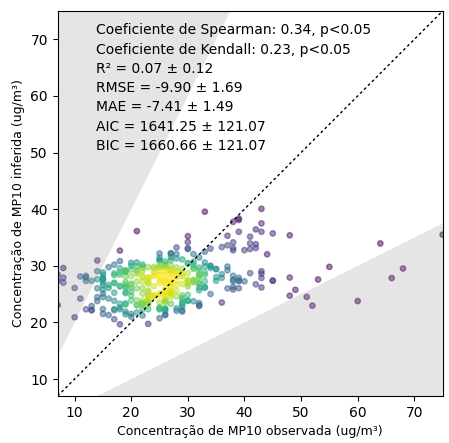
\includegraphics[width=\textwidth]{chapters/4-CALIBRAÇÃO MÚLTIPLOS SENSORES/Figuras/MP10-co-o31-o32-pm10-Multilinear-Regression.png}
        \caption{Utilizando modelo de regressão linear multivariado com variáveis independentes: leituras de sensores CO-B4, OX-B431 (1 e 2) e sensor de \acrshort{mp10} OPC-N3}
        \label{fig:data-co-o31-o31-pm10-reference-PM10-corr-MLR}
    \end{subfigure}
    \hfill
    \begin{subfigure}{0.49\textwidth}
        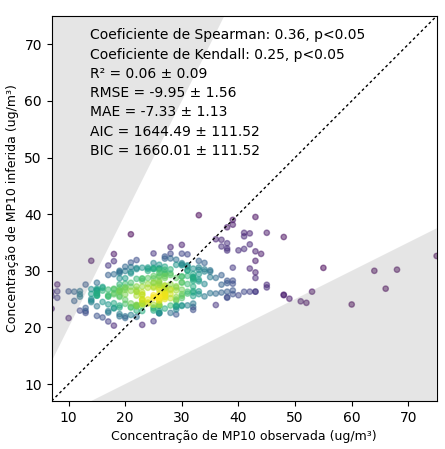
\includegraphics[width=\textwidth]{chapters/4-CALIBRAÇÃO MÚLTIPLOS SENSORES/Figuras/MP10-o31-o32-pm10-Multilinear-Regression.png}
        \caption{Utilizando modelo de regressão linear multivariado com variáveis independentes: leituras de sensores OX-B431 (1 e 2) e sensor de \acrshort{mp10} OPC-N3}
        \label{fig:data-o31-o32-pm10-reference-PM10-corr-RF}
    \end{subfigure}
\end{figure}
